% Options for packages loaded elsewhere
% Options for packages loaded elsewhere
\PassOptionsToPackage{unicode}{hyperref}
\PassOptionsToPackage{hyphens}{url}
\PassOptionsToPackage{dvipsnames,svgnames,x11names}{xcolor}
%

\documentclass[
  a4paper, 
  twoside,
  review
]{article}
\usepackage{xcolor}
\usepackage{amsmath,amssymb}
\setcounter{secnumdepth}{5}
\usepackage{iftex}
\ifPDFTeX
  \usepackage[T1]{fontenc}
  \usepackage[utf8]{inputenc}
  \usepackage{textcomp} % provide euro and other symbols
\else % if luatex or xetex
  \usepackage{unicode-math} % this also loads fontspec
  \defaultfontfeatures{Scale=MatchLowercase}
  \defaultfontfeatures[\rmfamily]{Ligatures=TeX,Scale=1}
\fi
\usepackage{lmodern}
\ifPDFTeX\else
  % xetex/luatex font selection
\fi
% Use upquote if available, for straight quotes in verbatim environments
\IfFileExists{upquote.sty}{\usepackage{upquote}}{}
\IfFileExists{microtype.sty}{% use microtype if available
  \usepackage[]{microtype}
  \UseMicrotypeSet[protrusion]{basicmath} % disable protrusion for tt fonts
}{}
\makeatletter
\@ifundefined{KOMAClassName}{% if non-KOMA class
  \IfFileExists{parskip.sty}{%
    \usepackage{parskip}
  }{% else
    \setlength{\parindent}{0pt}
    \setlength{\parskip}{6pt plus 2pt minus 1pt}}
}{% if KOMA class
  \KOMAoptions{parskip=half}}
\makeatother
% Make \paragraph and \subparagraph free-standing
\makeatletter
\ifx\paragraph\undefined\else
  \let\oldparagraph\paragraph
  \renewcommand{\paragraph}{
    \@ifstar
      \xxxParagraphStar
      \xxxParagraphNoStar
  }
  \newcommand{\xxxParagraphStar}[1]{\oldparagraph*{#1}\mbox{}}
  \newcommand{\xxxParagraphNoStar}[1]{\oldparagraph{#1}\mbox{}}
\fi
\ifx\subparagraph\undefined\else
  \let\oldsubparagraph\subparagraph
  \renewcommand{\subparagraph}{
    \@ifstar
      \xxxSubParagraphStar
      \xxxSubParagraphNoStar
  }
  \newcommand{\xxxSubParagraphStar}[1]{\oldsubparagraph*{#1}\mbox{}}
  \newcommand{\xxxSubParagraphNoStar}[1]{\oldsubparagraph{#1}\mbox{}}
\fi
\makeatother


\usepackage{longtable,booktabs,array}
\usepackage{calc} % for calculating minipage widths
% Correct order of tables after \paragraph or \subparagraph
\usepackage{etoolbox}
\makeatletter
\patchcmd\longtable{\par}{\if@noskipsec\mbox{}\fi\par}{}{}
\makeatother
% Allow footnotes in longtable head/foot
\IfFileExists{footnotehyper.sty}{\usepackage{footnotehyper}}{\usepackage{footnote}}
\makesavenoteenv{longtable}
\usepackage{graphicx}
\makeatletter
\newsavebox\pandoc@box
\newcommand*\pandocbounded[1]{% scales image to fit in text height/width
  \sbox\pandoc@box{#1}%
  \Gscale@div\@tempa{\textheight}{\dimexpr\ht\pandoc@box+\dp\pandoc@box\relax}%
  \Gscale@div\@tempb{\linewidth}{\wd\pandoc@box}%
  \ifdim\@tempb\p@<\@tempa\p@\let\@tempa\@tempb\fi% select the smaller of both
  \ifdim\@tempa\p@<\p@\scalebox{\@tempa}{\usebox\pandoc@box}%
  \else\usebox{\pandoc@box}%
  \fi%
}
% Set default figure placement to htbp
\def\fps@figure{htbp}
\makeatother





\setlength{\emergencystretch}{3em} % prevent overfull lines

\providecommand{\tightlist}{%
  \setlength{\itemsep}{0pt}\setlength{\parskip}{0pt}}



 
\usepackage[]{natbib}
\bibliographystyle{region}


\usepackage{region,hyperref,multirow}
\definecolor{mypink}{RGB}{219, 48, 122}
\makeatletter
\@ifpackageloaded{caption}{}{\usepackage{caption}}
\AtBeginDocument{%
\ifdefined\contentsname
  \renewcommand*\contentsname{Table of contents}
\else
  \newcommand\contentsname{Table of contents}
\fi
\ifdefined\listfigurename
  \renewcommand*\listfigurename{List of Figures}
\else
  \newcommand\listfigurename{List of Figures}
\fi
\ifdefined\listtablename
  \renewcommand*\listtablename{List of Tables}
\else
  \newcommand\listtablename{List of Tables}
\fi
\ifdefined\figurename
  \renewcommand*\figurename{Figure}
\else
  \newcommand\figurename{Figure}
\fi
\ifdefined\tablename
  \renewcommand*\tablename{Table}
\else
  \newcommand\tablename{Table}
\fi
}
\@ifpackageloaded{float}{}{\usepackage{float}}
\floatstyle{ruled}
\@ifundefined{c@chapter}{\newfloat{codelisting}{h}{lop}}{\newfloat{codelisting}{h}{lop}[chapter]}
\floatname{codelisting}{Listing}
\newcommand*\listoflistings{\listof{codelisting}{List of Listings}}
\makeatother
\makeatletter
\makeatother
\makeatletter
\@ifpackageloaded{caption}{}{\usepackage{caption}}
\@ifpackageloaded{subcaption}{}{\usepackage{subcaption}}
\makeatother
\usepackage{bookmark}
\IfFileExists{xurl.sty}{\usepackage{xurl}}{} % add URL line breaks if available
\urlstyle{same}
\hypersetup{
  pdftitle={Regional growth, convergence, and spatial spillovers in India:},
  pdfauthor={Carlos Mendez; Sujana Kabiraj; Jiaqi Li},
  pdfkeywords={Reproducible research, Nighttime lights, Regional
convergence, Spatial spillovers, Spatial Durbin model, India},
  colorlinks=true,
  linkcolor={blue},
  filecolor={Maroon},
  citecolor={Blue},
  urlcolor={blue},
  pdfcreator={LaTeX via pandoc}}




\title{Regional growth, convergence, and spatial spillovers in India:}
\usepackage{etoolbox}
\makeatletter
\providecommand{\subtitle}[1]{% add subtitle to \maketitle
  \apptocmd{\@title}{\par {\large #1 \par}}{}{}
}
\makeatother
\subtitle{A reproducible view from outer space}
\author{%
Carlos Mendez\parnote{Nagoya University, Nagoya, Japan}, 
Sujana Kabiraj\parnote{Shiv Nadar University, Greater Noida, India}, 
Jiaqi Li\parnote{Nagoya University, Nagoya, Japan}}
\date{}

\setcounter{page}{999}
\renewcommand{\thepage}{\arabic{page}}  % L for Letters, R for Resources, E for Editorial
\jvol{1} 
\jnum{1} 
\jyear{2020} 
\jpages{999--999} 
\jauthor{MISSING} 
\received{February 4, 2026} 
\accepted{} 

\jdoi{10.18335/region.v??i??.???} 

\setlength{\parskip}{0pt plus1pt}
\setlength{\parindent}{15pt}

% %\bibliographystyle{plainnat}
\bibpunct{(}{)}{,}{a}{}{,}   % % changes formatting in natbib, see http://merkel.zoneo.net/Latex/natbib.php
% % It can be moved into the package call!

%%%%%%%%%%% GM inserted %%%%%%%%%%%%%%%
\usepackage[breakable]{tcolorbox}

% prompt
\makeatletter
\newcommand{\boxspacing}{\kern\kvtcb@left@rule\kern\kvtcb@boxsep}
\makeatother
\newcommand{\prompt}[4]{
	\ttfamily\llap{{\color{#2}[#3]:\hspace{3pt}#4}}\vspace{-\baselineskip}
}

\definecolor{incolor}{HTML}{303F9F}
\definecolor{outcolor}{HTML}{D84315}
\definecolor{cellborder}{HTML}{CFCFCF}
\definecolor{cellbackground}{HTML}{F7F7F7}
\definecolor{celloutborder}{HTML}{FFAFAF}
\definecolor{celloutbackground}{HTML}{F7E7E7}

\newcounter{code}
%%%%%%%%%%%%%%%%%%%%%%%%%%%%%%%%%%%%%%%

\newenvironment{ROutput}{\definecolor{shadecolor}{HTML}{F7E7E7}\begin{snugshade}}{\end{snugshade}}
\newenvironment*{RInput}{}{}
\begin{document}
\maketitle
\begin{abstract}
Using satellite nighttime light data as a proxy for economic activity,
Chanda and Kabiraj (2020, World Development) studied regional growth and
convergence across 520 districts in India. Based on a reproducible
open-science approach, this article builds on their work by confirming
and extending their main findings on three fronts. First, we illustrate
regional convergence patterns using an interactive web-based tool for
satellite image visualization. Second, we assess the degree of spatial
dependence in their main econometric specification. Third, we employ a
spatial Durbin model to measure the role of spatial spillovers in the
convergence process. Our results indicate that spatial spillovers
increase the estimated speed of regional convergence. Overall, the
results highlight the role of spatial dependence in regional convergence
through the lens of satellite imagery, interactive visualizations, and
spillover modeling.
\end{abstract}


\section{Introduction}\label{introduction}

Regional economic growth and convergence are key concerns in developing
countries, particularly in large federal states like India where spatial
inequalities can threaten social cohesion and political stability.
However, studying regional convergence patterns in developing countries
has been historically challenging due to limited availability of
consistent economic data at subnational administrative levels. The
emergence of satellite nighttime light data as a proxy for economic
activity has created new opportunities to analyze regional growth
dynamics at granular geographic scales.

In an important contribution,
\citet{chanda_kabiraj_district_convergence} leveraged nighttime light
data to document evidence of regional convergence across 520 districts
in India between 1996 and 2010. Their analysis showed that poorer
districts grew faster than richer ones during this period, suggesting a
gradual reduction in spatial inequalities. However, their econometric
approach did not account for potential spatial spillovers in the
convergence process---the possibility that a district's growth
trajectory might be influenced not only by its own initial conditions
but also by those of its neighbors.

In this context, this paper confirms and extends the study of
\citet{chanda_kabiraj_district_convergence} in three key methodological
directions. First, we develop an interactive web-based visualization
tool that allows researchers to dynamically explore spatial and temporal
patterns in the nighttime light data. This tool facilitates the
identification of converging regions and growth hotspots that may be
difficult to detect in static representations. Second, we formally test
for spatial dependence in both the dependent and independent variables
of the convergence equations, highlighting that spatial autocorrelation
is a relevant feature of satellite data and the regional convergence
process. Third, we employ a spatial Durbin model that explicitly
accounts for spatial spillovers, quantifying how neighborhood effects
influence the speed of regional convergence.

Our results yield three main findings that contribute to the
understanding of regional convergence in India. First, interactive
visualization tools reveal clear spatial patterns in both the initial
distribution and subsequent growth of nighttime lights. Second, formal
tests of spatial dependence indicate that district-level economic
trajectories are not independent of their neighbors. Third, accounting
for spatial spillovers through the spatial Durbin model shows that the
total convergence effect is substantially larger than previous
non-spatial estimates would suggest. Specifically, spatial spillovers
appear to accelerate the convergence process by creating additional
channels through which lagging regions can catch up.

These findings have important implications for both research methodology
and policy design. Methodologically, they suggest that conventional
non-spatial approaches may underestimate the speed of regional
convergence by failing to account for inter-district spillovers. From a
policy perspective, they suggest that the benefits of place-based
development interventions may extend beyond target districts through
spatial multiplier effects, potentially increasing their
cost-effectiveness. The results also highlight the value of new data
sources and methodological tools in advancing our understanding of
regional economic dynamics in developing countries.

The rest of this article is organized as follows. Section 2 provides an
overview of the data and methods, describing our use of nighttime light
data as a proxy for economic activity and introducing the spatial Durbin
model that forms the basis of our empirical strategy. We also detail our
methodological extensions related to interactive visualizations, spatial
dependence testing, and spillover modeling. Section 3 presents our
empirical results, beginning with an interactive exploration of regional
convergence patterns, followed by formal tests of spatial dependence,
and concluding with estimates of direct and indirect convergence effects
from the spatial Durbin model. Finally, Section 4 offers some concluding
remarks.

\section{Data and methods}\label{data-and-methods}

\subsection{Data: Nighttime lights as a proxy for economic
activity}\label{data-nighttime-lights-as-a-proxy-for-economic-activity}

One of the key challenges in studying economic growth in developing
countries like India is the limited availability and reliability of data
on aggregate economic activity at finer administrative levels beyond the
state level. To address this issue, a growing body of literature,
pioneered by \citet{henderson_storeygard_weil_lights}, has utilized
satellite nighttime light data as a proxy for economic activity at
subnational levels.

Nighttime light (hereafter NTL) data have been widely used to
investigate economic growth and convergence across national and
subnational regions in various countries. For instance,
\citet{adhikari_dhital_decentralization} examine the impact of
decentralization on regional convergence using NTL data, while
\citet{pinkovskiy_salaimartin_lights_poverty} use NTL data to adjudicate
between national accounts and household surveys, finding that national
accounts better capture aggregate economic growth. Similarly,
\citet{lessmann_seidel_regional_inequality} leverage NTL data to
estimate GDP per capita and income inequality globally. More broadly,
\citet{gennaioli_etal_growth_regions} study regional convergence using
per capita income data from 1,528 subnational regions across 83
countries, finding a convergence rate of about 2\% per year.

NTL data have been extensively used in India across various contexts.
For example, \citet{cook_shah_nregs} use NTL data to analyze the impact
of public welfare programs, while \citet{jha_talathi_colonial_india}
examine the effects of colonial institutions, and
\citet{chanda_cook_demonetization} investigate the impact of
demonetization. \citet{beyer_jain_sinha_covid} employ NTL data to study
the effects of COVID-19. In the context of convergence studies,
\citet{chakravarty_dehejia_gst} document significant regional
disparities in India using NTL data and caution that GST may further
exacerbate them, while \citet{chanda_kabiraj_district_convergence}
highlights district-level convergence.

Our study builds on \citet{chanda_kabiraj_district_convergence}.
Following their approach, we use the per capita growth in nighttime
lights as the dependent variable and the initial nighttime lights per
capita as the primary variable of interest. These variables are derived
from NTL data released by the National Geophysical Data Center (NGDC),
based on observations from the DMSP/OLS satellites spanning the period
from 1996 to 2010. To mitigate the issue of top-coding in NTL data, the
NGDC released ``radiance-calibrated'' nighttime lights for eight
specific years within this period. This dataset employs high
magnification settings for low-light regions and low magnification
settings for brightly lit areas. For this study, we utilize the
``radiance-calibrated'' nighttime lights data.\footnote{Following
  \citet{chanda_kabiraj_district_convergence}, our sample consists of
  520 districts (out of a possible 593). There were 593 districts in
  2001, which rose to 640 districts in the 2011 census. To match the
  districts among two census files, we summed up the carved-out
  districts with their origin districts in the 2011 census files. Eight
  districts among 47 new districts were created by carving out some
  areas from multiple districts. Those new districts along with their
  multiple-origin districts were dropped from our sample. We dropped all
  the districts in the state of Assam where more than 50\% of districts
  were created in that manner.}

\subsection{Jupyter and Quarto for reproducible open
science}\label{jupyter-and-quarto-for-reproducible-open-science}

Jupyter notebooks have become an essential tool for reproducible open
science, as they allow researchers to integrate executable code,
explanatory narrative, and computational outputs within a single,
self-contained document \citep{kluyver_jupyter}. This integration
ensures that every step of the analytical workflow---from data ingestion
and processing to statistical modeling and visualization---is
transparently documented and can be independently verified by other
researchers. Unlike traditional workflows where code, results, and
interpretation are separated across different files and software
environments, Jupyter notebooks preserve the complete chain of reasoning
in a format that can be shared, inspected, and re-executed. In this
article, we employ Jupyter notebooks with three distinct computational
kernels---Python, R, and Stata---to document our data processing,
analysis, and visualization steps, enabling readers and reviewers to
trace each result back to the code that produced it. The Python and R
notebooks can be executed in the cloud using Google Colab, further
lowering the barriers to replication by eliminating the need for local
software installation. While Stata is not open-source software, its
integration with the Jupyter environment provides a rich interactive
interface that brings the same benefits of literate programming and
transparent documentation to proprietary statistical software
\citep{knuth_literate}.

Quarto is an open-source scientific and technical publishing system that
extends the capabilities of computational notebooks into a comprehensive
manuscript preparation framework \citep{allaire_quarto}. Its
single-source publishing paradigm enables researchers to generate
multiple output formats---including HTML for interactive web-based
dissemination, PDF for formal journal submission, Word documents for
collaborative editing, and JATS XML for archival and indexing
purposes---from a single source file. This approach ensures consistency
across all versions of a document, eliminating discrepancies that can
arise when maintaining separate files for different output formats. By
providing a unified authoring environment that natively supports
cross-references, citations, mathematical notation, and embedded
computational results, Quarto substantially reduces the technical
barriers to producing publication-quality research outputs that adhere
to open-access and reproducibility standards.

The combination of Jupyter notebooks and Quarto's manuscript framework
creates an effective infrastructure for reproducible research. In this
article, all computational analyses are embedded in Jupyter notebooks
that are directly linked to the main text, allowing readers to inspect
the code alongside the results it produces. Quarto's embed functionality
enables us to pull specific figures, tables, and results from these
notebooks into the manuscript, ensuring that every empirical finding
presented in the text is traceable to its underlying computation. All
data processing and analysis steps are documented in the notebooks, and
we provide access to the raw data and code through a public repository.
By adopting this integrated reproducible research framework, we aim to
contribute to the open science movement and encourage other researchers
to build upon our work by ensuring transparency and verifiability of our
findings \citep{peng_reproducible}.

\subsection{Google Earth Engine for interactive spatial
visualizations}\label{google-earth-engine-for-interactive-spatial-visualizations}

Interactive visualizations of nighttime lights imagery offer distinct
methodological advantages over static representations, particularly when
analyzing temporal and spatial heterogeneity in economic activity
\citep{donaldson_storeygard_remotesensing}. The dynamic nature of these
visualizations enables researchers to simultaneously examine multiple
dimensions of the data, including temporal variations in light
intensity, the spatial distribution of economic activity, and the
relationship between nighttime lights and other georeferenced variables.
This interactivity is especially valuable when investigating economic
phenomena that exhibit significant spatial and temporal variation, such
as urbanization patterns, economic shocks, or regional development
disparities. The ability to dynamically adjust visualization parameters,
such as temporal ranges, spatial scales, and light intensity thresholds,
allows for more nuanced exploration of economic patterns that might be
obscured in static representations.

Google Earth Engine (GEE) substantially reduces the computational and
technical barriers to creating such interactive visualizations, offering
a particularly advantageous platform for economic research utilizing
nighttime lights data \citep{gorelick_gee}. The platform's browser-based
integrated development environment facilitates the creation of
interactive web applications without requiring extensive infrastructure
or specialized software installation. This capability is especially
valuable for reproducible research, as it enables the development of web
applications that can be shared with other researchers or stakeholders,
allowing them to interact with the data and verify findings
independently. The platform's ability to handle large-scale geospatial
computations server-side, combined with its extensive catalog of
pre-processed nighttime lights datasets, including the DMSP-OLS and
VIIRS collections, significantly streamlines the workflow from raw data
to interactive visualization \citep{tamiminia_gee_review}. This
computational efficiency is particularly beneficial when analyzing long
time series or large geographic areas, which would be computationally
intensive using traditional desktop-based approaches.

Interactive visualizations of nighttime lights data are particularly
useful for identifying and analyzing patterns of regional convergence in
luminosity, providing visual insights into economic convergence
processes. Through dynamic visualization tools, researchers can track
the evolution of light intensity across regions over time, effectively
identifying areas that exhibit catch-up growth patterns - where
initially dim regions progressively converge toward the luminosity
levels of their brighter counterparts.

\subsection{Modeling regional
convergence}\label{modeling-regional-convergence}

In neoclassical growth models, such as the Solow model, it is argued
that the per capita growth rate should be negatively correlated with a
region's initial endowment primarily due to diminishing returns to
capital \citep{solow_growth}. Specifically, poorer regions, assuming
similar technology and preferences, are expected to experience higher
growth rates compared to their wealthier counterparts. Consequently,
over the long run, regions with similar characteristics should converge
to a common steady state. We examine such convergence (denoted by
\textbf{\(\beta\)-convergence}) employing a growth regressions framework
in the tradition of \citet{barro_sala_convergence}.
Equation~\ref{eq-matrix-form-abs} analyzes absolute convergence.

\begin{equation}\phantomsection\label{eq-matrix-form-abs}{
\boldsymbol{g_t} =  \beta_1 \boldsymbol{x_{t-1}} +  \boldsymbol{\varepsilon_t}
}\end{equation}

where \(\boldsymbol{g_t}\) represents an \(N\text{-by-}1\) vector of
observations on NTL growth for each of the \(N\) regions over the period
\(t\) and \(\boldsymbol{x_{t-1}}\) represents an \(N\text{-by-}1\)
vector of observations on the initial (log) level of NTL. The scalar
\(\beta_1\) is a regression coefficient that indicates the direction and
strength of regional convergence. Finally,
\(\boldsymbol{\varepsilon_t}\) represents a vector of idiosyncratic
error terms.

While absolute convergence implies that districts converge to a common
steady state, regions may differ in various aspects such as geography,
socio-economic conditions, and policy implementation. To account for
these differences, we include state dummies in our analysis to examine
whether heterogeneity in state-specific institutions and policies
influences the rate of convergence. Additionally, we control for the
initial share of unlit pixels in districts to address any potential
under-coding in NTL data.

To further explore the determinants of district-level growth rates, we
incorporate a range of geo-climatic controls alongside initial
district-specific conditions related to demographics, human capital, and
infrastructure. Equation~\ref{eq-matrix-form-cond} explores conditional
convergence.

\begin{equation}\phantomsection\label{eq-matrix-form-cond}{
\boldsymbol{g_t} =  \beta_1 \boldsymbol{x_{t-1}} + \boldsymbol{X_t} \boldsymbol{\alpha}  + \boldsymbol{\varepsilon_t}
}\end{equation}

Here, the matrix \(\boldsymbol{X_t}\) is a \(N\text{-by-}k\) collection
of observations on control variables for each region. The vector
\(\boldsymbol{\alpha}\), with dimensions \(k \times 1\), captures the
regression coefficients for these variables. The control variables are
listed in Table A.1 in \citet{chanda_kabiraj_district_convergence}.

\subsection{Spatial dependence
testing}\label{spatial-dependence-testing}

The analysis of regional convergence using nighttime light data requires
explicit consideration of spatial dependence patterns across Indian
districts. Spatial dependence---the tendency for observations at nearby
locations to be more similar than those at distant locations---can arise
from spatial spillovers, shared geographic conditions, or inter-regional
economic linkages \citep{anselin_spatial_analysis}. If present and
unaccounted for, spatial dependence can lead to biased parameter
estimates and invalid inference in standard regression models. To
formally test for such spatial relationships, we employ the Global
Moran's I statistic and Local Indicators of Spatial Association (LISA),
applied to the main variables of Equation~\ref{eq-matrix-form-cond}.

The Global Moran's I statistic, originally proposed by
\citet{moran_spatial_autocorrelation}, is the most widely used measure
of spatial autocorrelation. It quantifies the overall degree of spatial
clustering among geographic units and can be expressed as:

\begin{equation}\phantomsection\label{eq-moran}{
I=\frac{n}{\sum_i \sum_j w_{ij}} \cdot \frac{\sum_i \sum_j w_{ij} \, z_i \, z_j}{\sum_i z_i^2}
}\end{equation}

where \(z_i\) represents the deviation of observation \(i\) from the
mean, \(w_{ij}\) denotes the spatial weight between units \(i\) and
\(j\), and \(n\) is the total number of observations. The Moran's I
statistic ranges from \(-1\) to \(+1\): positive values indicate
positive spatial autocorrelation (spatial clustering, where similar
values tend to be located near each other), values near zero suggest
spatial randomness, and negative values indicate spatial dispersion
(where dissimilar values are neighbors). Statistical significance is
assessed through a permutation-based inference approach that compares
the observed statistic against a reference distribution generated by
randomly reassigning values across locations.

While the Global Moran's I provides a single summary measure of overall
spatial dependence, it does not reveal where significant clusters or
outliers are located. To address this limitation, \citet{anselin_lisa}
proposed Local Indicators of Spatial Association (LISA), which decompose
the global statistic into contributions from each individual
observation. The local Moran's I for observation \(i\) is defined as:

\begin{equation}\phantomsection\label{eq-lisa}{
I_i = z_i \sum_j w_{ij} \, z_j
}\end{equation}

where the summation is over the neighbors of \(i\) as defined by the
spatial weight matrix. This local statistic classifies each observation
into one of four categories based on the relationship between a
location's value and those of its neighbors: High-High (HH), where a
high-value location is surrounded by high-value neighbors; Low-Low (LL),
where a low-value location is surrounded by low-value neighbors;
High-Low (HL), a spatial outlier where a high-value location is
surrounded by low-value neighbors; and Low-High (LH), the opposite
spatial outlier. Taken together, the HH and LL categories identify
spatial clusters, while the HL and LH categories identify spatial
outliers. Statistical significance of each local statistic is assessed
through conditional permutation tests, with only statistically
significant locations (typically at \(p < 0.05\)) reported in the LISA
cluster maps.

The specification of the spatial weights matrix \(\mathbf{W}\) is
crucial for capturing the underlying spatial structure. We employ a
\(k\)-nearest neighbors weight matrix with \(k = 6\), whereby for each
district, the six geographically closest districts are identified as its
neighbors:

\[
\mathbf{W}=\left[\begin{array}{ccccc}
w_{11} & w_{12} & w_{13} & \cdots & w_{1n} \\
w_{21} & w_{22} & w_{23} & \cdots & w_{2n} \\
\vdots & \vdots & \vdots & w_{ij} & \vdots \\
w_{n1} & w_{n2} & w_{n3} & \cdots & w_{nn}
\end{array}\right]
\]

where \(w_{ij} = 1\) if district \(j\) is among the six nearest
neighbors of district \(i\), and \(w_{ij} = 0\) otherwise. Following
standard practice, we row-normalize the weights matrix so that each row
sums to one, ensuring that the spatial lag of a variable represents the
average value among a district's neighbors.

The detection of significant spatial dependence would justify the use of
spatial econometric techniques. In particular,
\citet{ertur_koch_spatial_growth} and \citet{fischer_spatial_mrw} argue
that the spatial Durbin model can appropriately account for spatial
spillovers in the convergence process. This methodological choice allows
us to distinguish between direct effects of district characteristics and
indirect effects operating through spatial channels
\citep{lesage_pace_spatial_econometrics}.

\subsection{Spatial spillover
modeling}\label{spatial-spillover-modeling}

Our spatial spillover modeling builds upon the spatial Solow growth
model developed by \citet{ertur_koch_spatial_growth} and
\citet{fischer_spatial_mrw}, which extends the traditional Solow
framework to account for technological interdependence across regions.
The model considers an economy of \(N\) subnational regions, each
characterized by a Cobb-Douglas production function with constant
returns to scale:

\begin{equation}\phantomsection\label{eq-production}{
Y_{i t}=A_{i t} K_{i t}^{\alpha_{K}} H_{i t}^{\alpha_{H}} L_{i t}^{1-\alpha_{K} -\alpha_{H}}
}\end{equation}

where \(Y_{it}\) represents output, \(K_{it}\) physical capital,
\(H_{it}\) human capital, \(L_{it}\) labor force, and \(A_{it}\) the
level of technological knowledge for region \(i\) at time \(t\). The
parameters \(\alpha_K\) and \(\alpha_H\) denote the output elasticities
with respect to physical and human capital, respectively. A key
innovation of this framework is the modeling of technological knowledge,
which incorporates both internal and external factors:

\begin{equation}\phantomsection\label{eq-technology}{
A_{i t}=\Omega_{t} k_{i t}^{\theta} h_{i t}^{\phi} \prod_{j \neq i}^{N} A_{j t}^{\rho W_{i j}}
}\end{equation}

This specification captures three distinct components of technological
progress:

\begin{itemize}
\tightlist
\item
  An exogenous component (\(\Omega_t\)) representing the common stock of
  knowledge across regions
\item
  An embodied component (\(k_{i t}^{\theta} h_{i t}^{\phi}\)) reflecting
  technology embedded in physical and human capital per worker
\item
  A spatial component (\(\prod_{j \neq i}^{N} A_{j t}^{\rho W_{i j}}\))
  capturing technological interdependence between regions
\end{itemize}

Based on this theoretical framework, \citet{ertur_koch_spatial_growth}
derived a spatial panel Durbin model that accounts for regional
spillovers across economies. Their model can be compactly written in
matrix notation as:

\begin{equation}\phantomsection\label{eq-matrix_form}{
\boldsymbol{g_t} =  \beta_1 \boldsymbol{x_{t-1}} + \boldsymbol{X_t} \boldsymbol{\alpha} + \beta_2 \boldsymbol{W} \boldsymbol{x_{t-1}} + \boldsymbol{W} \boldsymbol{X_t} \boldsymbol{\gamma} + \lambda \boldsymbol{W} \boldsymbol{g_t}  + \boldsymbol{\varepsilon_t}
}\end{equation}

In this model, \(\boldsymbol{g_t}\) represents an \(N\text{-by-}1\)
vector of observations on NTL growth for each of the \(N\) regions over
the period \(t\) and \(\boldsymbol{x_{t-1}}\) represents an
\(N\text{-by-}1\) vector of observations on the initial (log) level of
NTL. The scalar \(\beta_1\) is a regression coefficient that indicates
the direction and strength of regional convergence. The matrix
\(\boldsymbol{X_t}\) is a \(N\text{-by-}k\) collection of observations
on control variables for each region. The vector
\(\boldsymbol{\alpha}\), with dimensions \(k \times 1\), captures the
regression coefficients for these variables. Additionally,
\(\boldsymbol{WX_t}\) denotes a \(N \times k\) matrix of spatially
lagged observations, composed of a linear combination of neighboring
values for the variables of interest in each region. The vector
\(\boldsymbol{\gamma}\) represents the regression coefficients
associated with these spatial lags. The terms
\(\boldsymbol{W} \boldsymbol{x_{t-1}}\) and
\(\boldsymbol{W} \boldsymbol{g_t}\) refer to \(N\text{-by-}1\) vectors
capturing the spatial lags of initial (log) level of NTL, and the NTL
growth, respectively. Finally, \(\boldsymbol{\varepsilon_t}\) represents
a vector of idiosyncratic error terms.

\section{Results}\label{results}

\subsection{Regional convergence: An interactive exploration from outer
space}\label{regional-convergence-an-interactive-exploration-from-outer-space}

Before presenting the regression results, we conduct three exercises to
visually illustrate the concepts of growth and convergence in nighttime
lights. First, we create an interactive map of India displaying regional
luminosity levels for 1996 and 2010.\footnote{The interactive web
  application is available at \url{https://bit.ly/india-rc-ntl}.}
Second, we examine absolute convergence by constructing a scatterplot
that depicts the relationship between per capita growth rates in
nighttime lights (1996--2010) and the initial per capita nighttime light
levels (1996) at the district level. Finally, we use case studies to
illustrate the nighttime light growth that occurred during our study
period. Focusing on some of the poorest regions in the country, we show
an increase in nighttime lights that aligns with our convergence
hypothesis.

\begin{figure}

\centering{

\pandocbounded{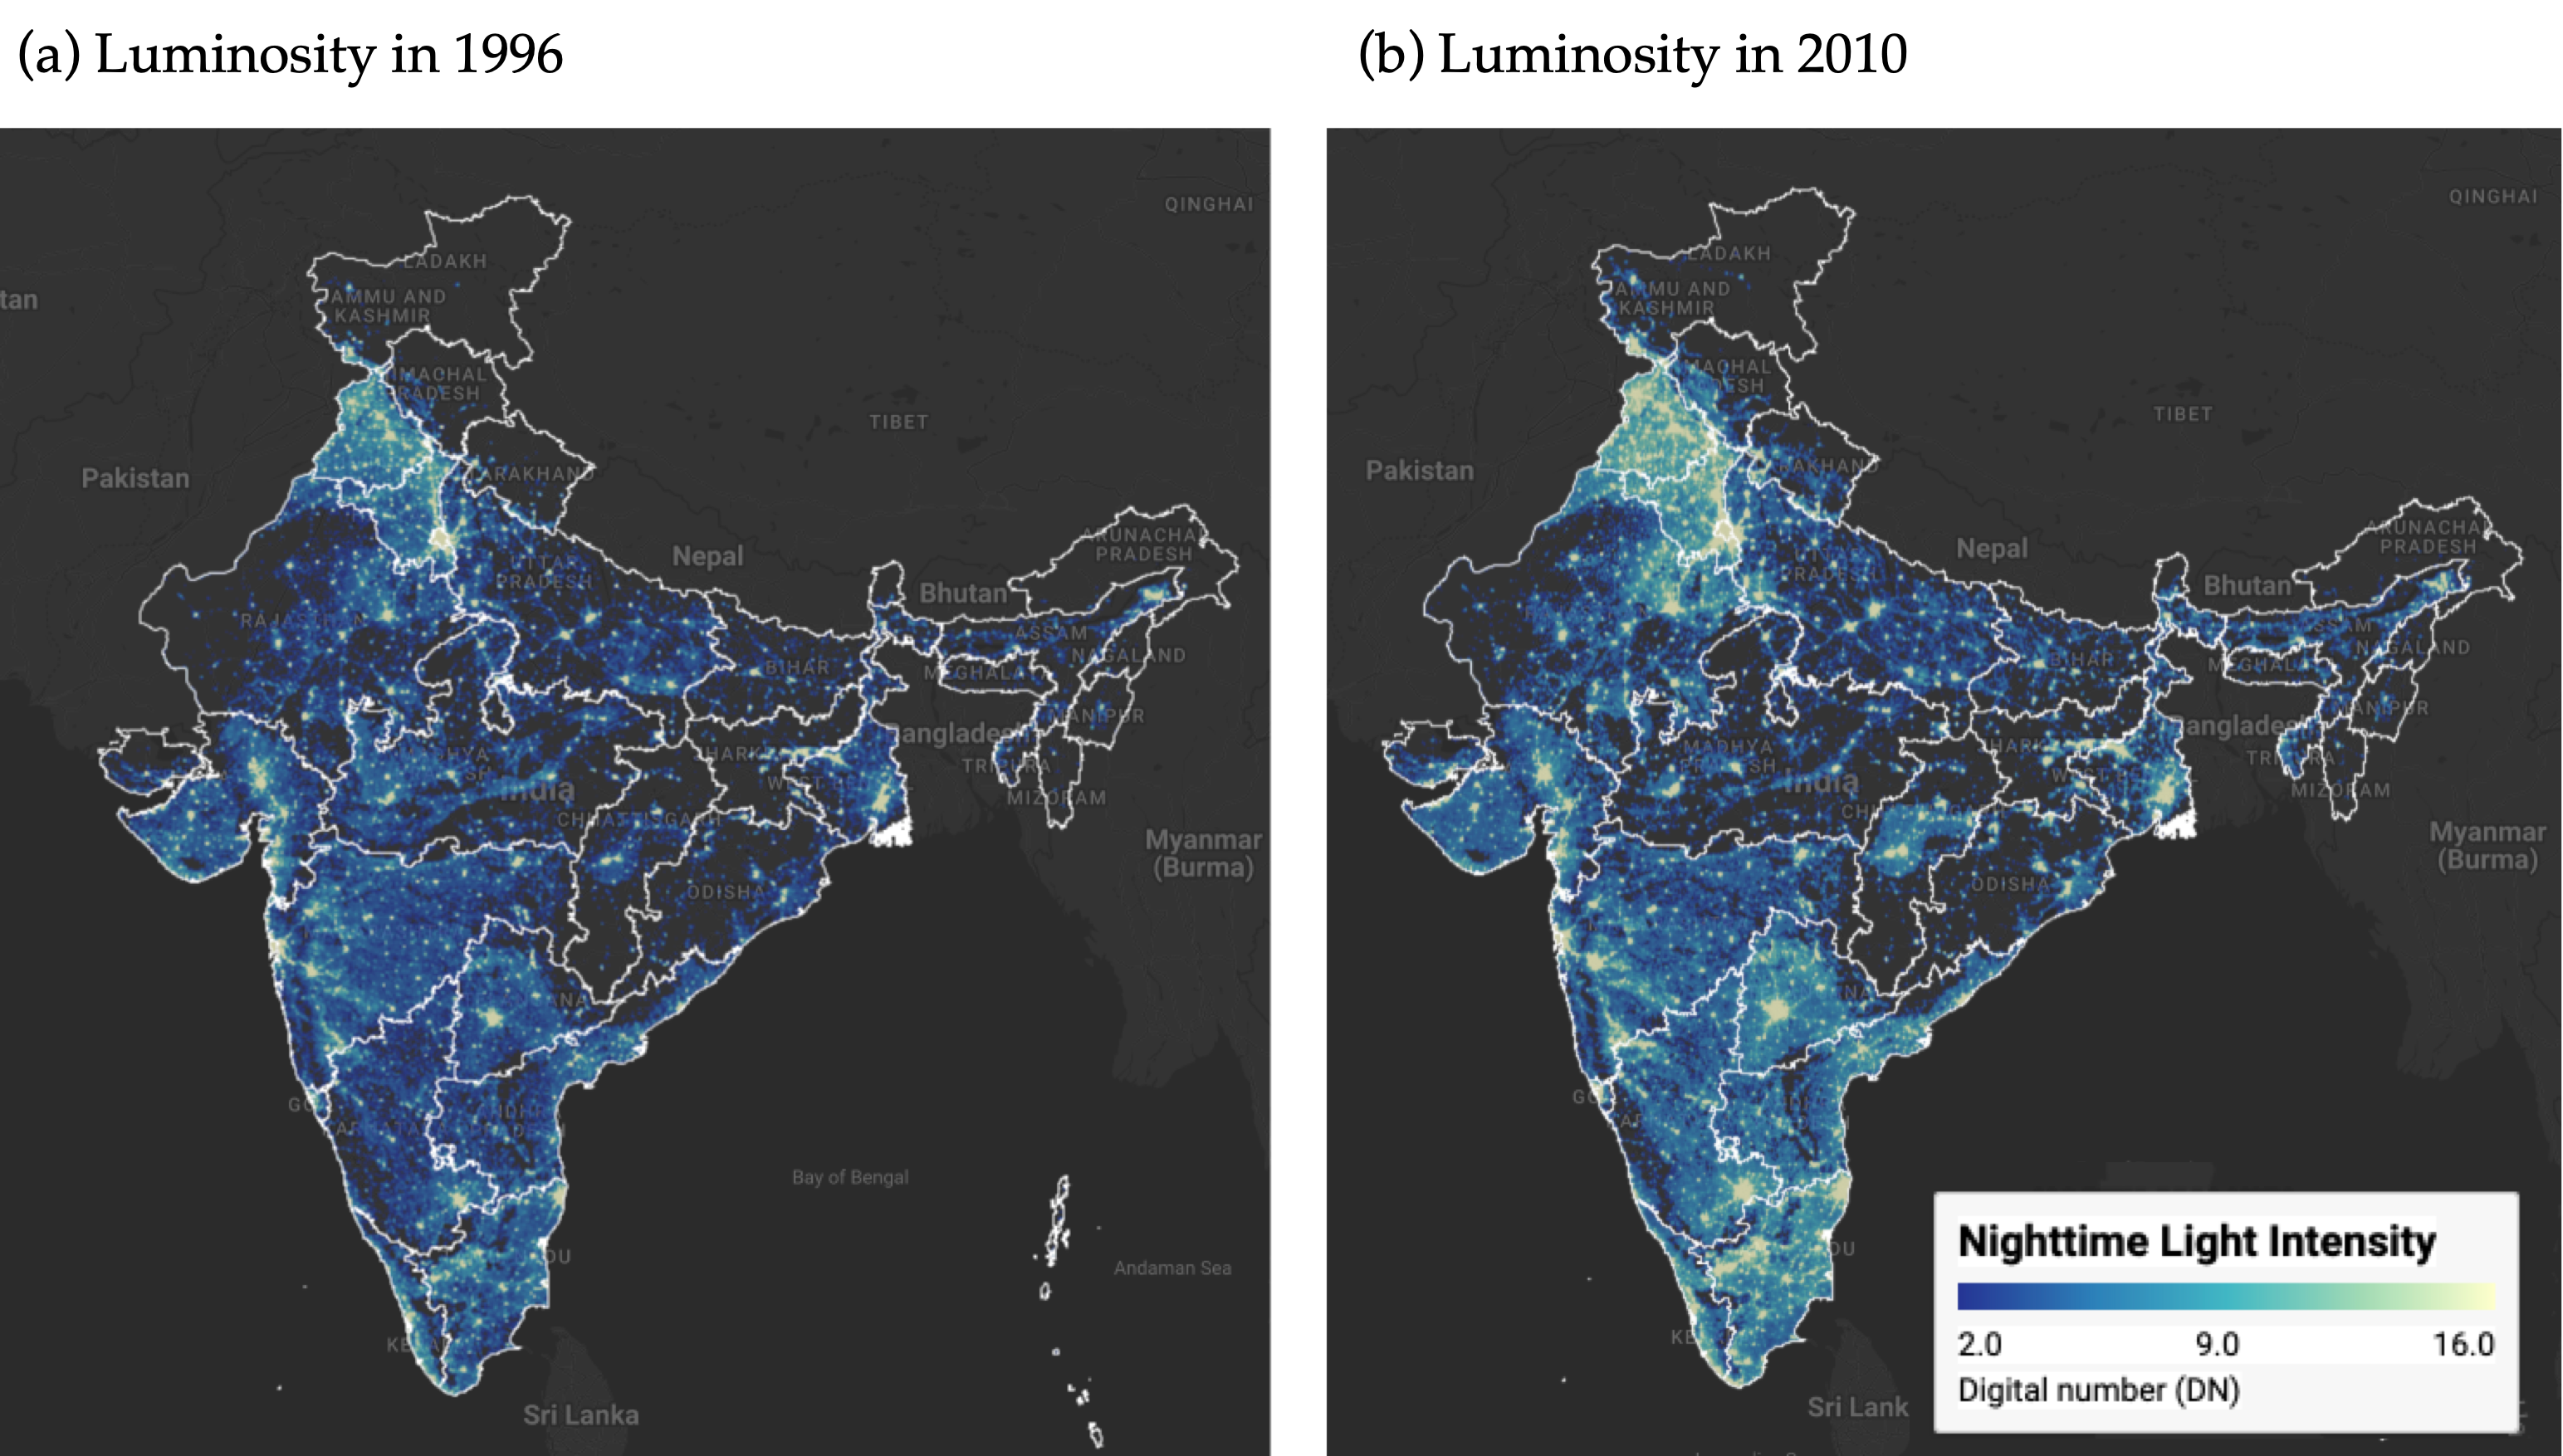
\includegraphics[keepaspectratio]{images/luminosity_map.png}}

}

\caption{\label{fig-map}Regional luminosity in India: 1996 vs 2010
Notes: Luminosity is measured in radiance-calibrated digital number (DN)
values from DMSP-OLS satellites. Interactive web application available
at https://bit.ly/india-rc-ntl . Source: Authors' visualization using
pre-processed luminosity images from the Earth Observation Group
(NOAA/NCEI). See \href{notebooks/c01_view_from_space.ipynb}{View from
outer space} notebook for source code.}

\end{figure}%

Figure 1 presents static maps (captured from our interactive maps) of
luminosity for our boundary years (1996 and 2010), using the same index
scale for comparison. The maps show a noticeable increase in brightness
across most parts of the country in 2010. Since nighttime lights serve
as a proxy for economic activity, this increase in luminosity reflects
economic growth over the period. Figure 2 illustrates the relationship
between per capita growth in nighttime lights and initial per capita
nighttime light levels. The scatterplot shows an inverse relationship,
suggesting a \(\beta\)-convergence rate of approximately 2\%, consistent
with Barro's ``Iron Law'' of convergence.

\begin{figure}

\centering{


\includegraphics[width=0.75\linewidth,height=\textheight,keepaspectratio]{images/luminosity_map2.png}

}

\caption{\label{fig-map2}Some illustrative examples of regional
convergence Notes: Luminosity is measured in radiance-calibrated digital
number (DN) values from DMSP-OLS satellites. Interactive web application
available at https://bit.ly/india-rc-ntl . Source: Authors'
visualization using pre-processed luminosity images from the Earth
Observation Group (NOAA/NCEI). See
\href{notebooks/c01_view_from_space.ipynb}{View from outer space}
notebook for source code.}

\end{figure}%

Next, we examine case studies of three economically disadvantaged states
in India to illustrate their growth patterns over the study period.
Among these, Bihar is the poorest, with a per capita income at 39.2\% of
the national average, while Uttar Pradesh and Chhattisgarh have per
capita incomes of 43.8\% and 52.3\% of the national average,
respectively.\footnote{The data are taken from a report by the Economic
  Advisory Council to the Prime Minister (EAC-PM), released on September
  18, 2024.} Figure 3 displays the change in luminosity in these three
states during our study period. Although these states remain among the
poorest, there is a noticeable increase in luminosity over the course of
the study.

\begin{figure}[H]

\centering{

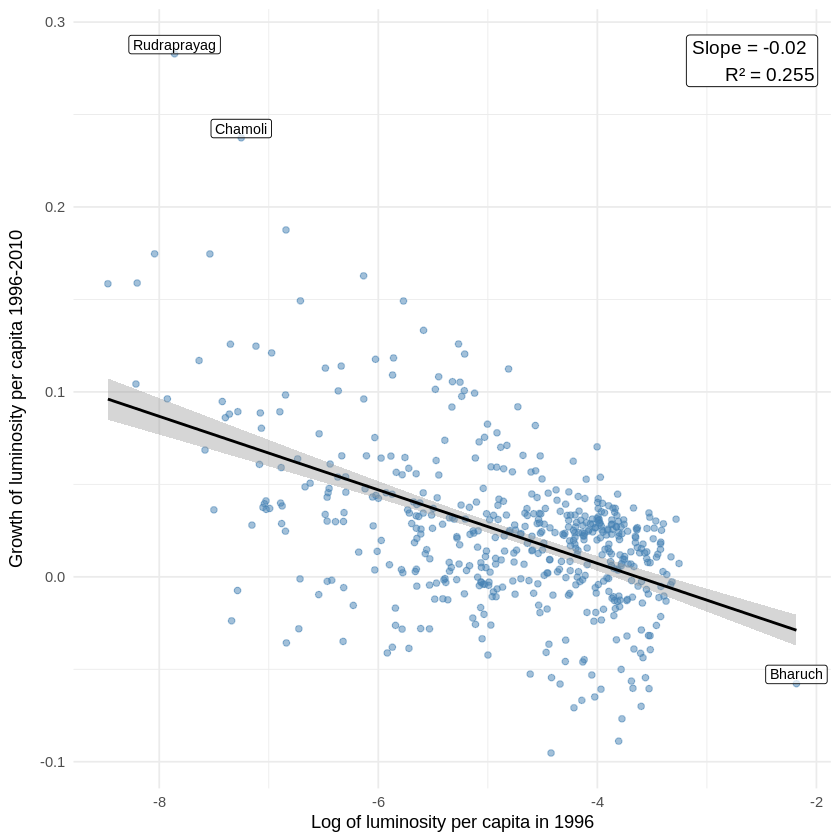
\includegraphics[width=4.375in,height=4.375in]{index_files/figure-latex/notebooks-c02_regional_convergence_sc-fig-convergence-output-2.png}

}

\caption{\label{fig-convergence}Regional luminosity convergence across
districts in India Notes: Each point represents one of the 520
districts. The regression line shows the estimated beta-convergence
relationship. Outlier districts are labeled. Source: Data from Chanda
and Kabiraj (2020). See
\href{notebooks/c02_regional_convergence_sc.ipynb}{Regional convergence}
notebook for source code.}

\end{figure}%

\textsubscript{Source:
\href{https://quarcs-lab.github.io/project2025s/notebooks/c02_regional_convergence_sc.ipynb.html\#cell-fig-convergence}{Setup}}

\subsection{Spatial dependence is a feature of the convergence
process}\label{spatial-dependence-is-a-feature-of-the-convergence-process}

Before proceeding with formal econometric analysis, it is instructive to
examine the spatial distribution of the variables under study.
Choropleth maps provide a natural tool for this purpose, as they allow
researchers to visualize how a variable of interest varies across
geographic units and to identify spatial patterns that may not be
apparent from summary statistics alone. Figure~\ref{fig-chorophleths}
presents the spatial distribution of initial luminosity per capita in
1996 and the subsequent growth rate of luminosity per capita over the
1996--2010 period across the 520 districts in our sample.

\begin{figure}[H]

\centering{

\pandocbounded{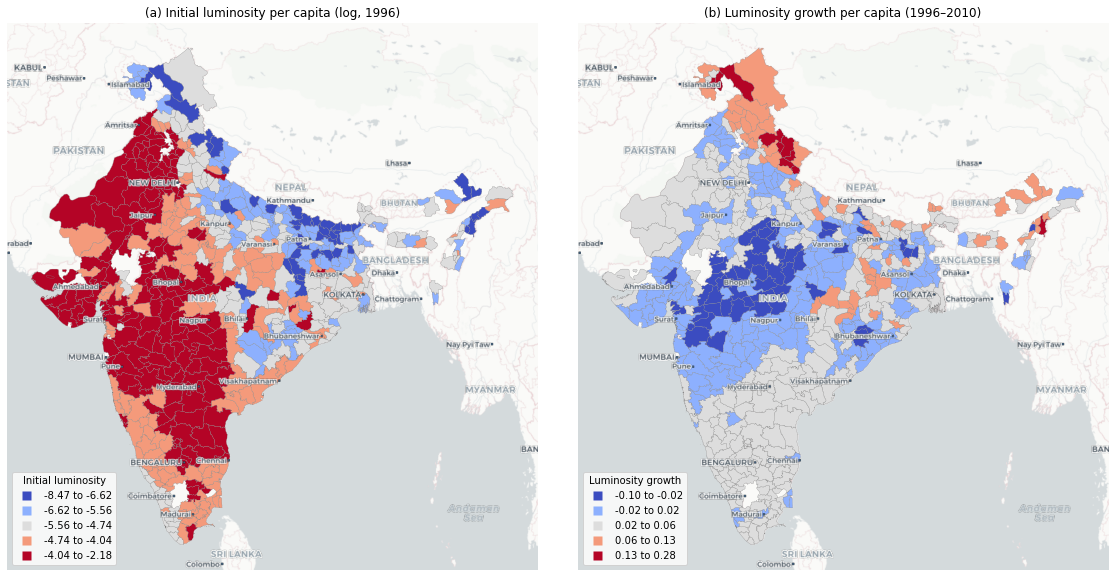
\includegraphics[keepaspectratio]{index_files/figure-latex/notebooks-c03_spatial_dependence_lisa-fig-chorophleths-output-1.png}}

}

\caption{\label{fig-chorophleths}Spatial distribution of initial
luminosity and luminosity growth Notes: Districts are classified into
five categories using Fisher-Jenks natural breaks. Panel (a) shows log
of luminosity per capita in 1996. Panel (b) shows luminosity growth per
capita over 1996--2010. Source: Data from Chanda and Kabiraj (2020). See
\href{notebooks/c03_spatial_dependence_lisa.ipynb}{Spatial dependence}
notebook for source code.}

\end{figure}%

\textsubscript{Source:
\href{https://quarcs-lab.github.io/project2025s/notebooks/c03_spatial_dependence_lisa.ipynb.html\#cell-fig-chorophleths}{Setup}}

The choropleth maps in Figure~\ref{fig-chorophleths} reveal a distinct
spatial pattern. Panel (a) shows that initial luminosity levels are
concentrated in specific geographic corridors, with higher values
clustered along western coastal areas while large portions of central
and eastern India exhibit substantially lower luminosity. Panel (b),
which displays the growth rate of luminosity per capita over the study
period, presents a pattern that is largely the inverse of the initial
distribution: districts that were initially bright tend to exhibit lower
growth rates, whereas districts that were initially dim tend to grow at
a faster rate. This spatial inversion provides a first visual indication
that regional convergence in India may have an important spatial
dimension.

While the choropleth maps visually suggest the presence of spatial
structures in both variables, a formal analysis of spatial dependence
requires the definition of a neighborhood for each district. This
neighborhood structure is specified through a spatial weight matrix,
which encodes the connectivity between geographic units. In this study,
we adopt a six nearest neighbors weight matrix, whereby for each of the
520 districts, the six geographically closest districts are identified
as its neighbors. This connectivity structure is visualized as a network
in Figure~\ref{fig-wmatrix6nn}, where each node represents a district
centroid and each edge connects a district to one of its six nearest
neighbors.

\begin{figure}[H]

\centering{

\pandocbounded{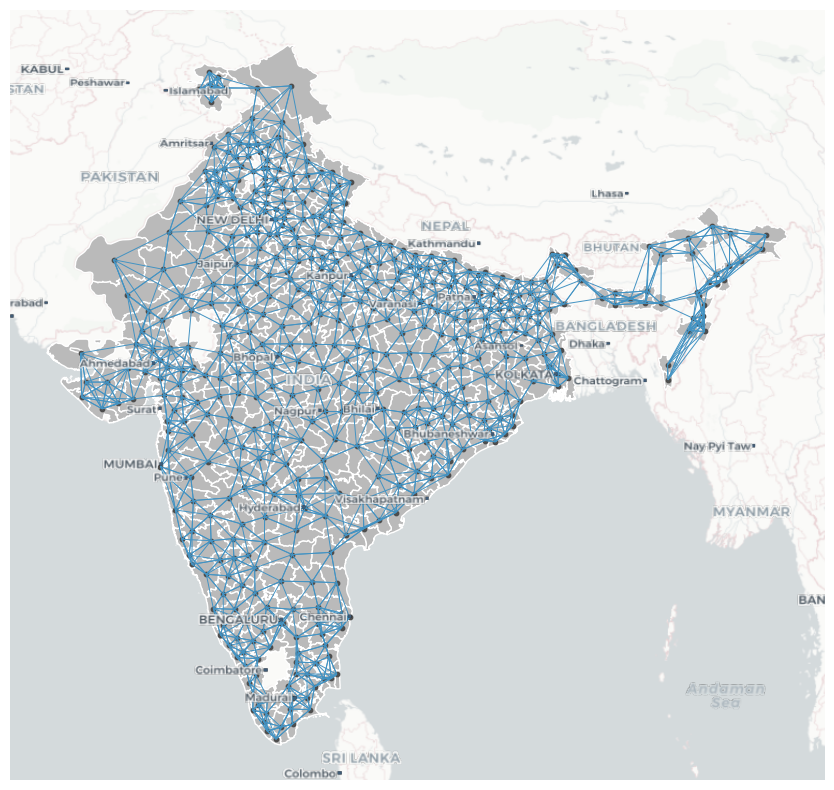
\includegraphics[keepaspectratio]{index_files/figure-latex/notebooks-c03_spatial_dependence_lisa-fig-wmatrix6nn-output-1.png}}

}

\caption{\label{fig-wmatrix6nn}Spatial connectivity structure based on
six nearest neighbors Notes: Each node represents a district centroid.
Each edge connects a district to one of its six geographically closest
neighbors. The weight matrix is row-standardized. Source: Data from
Chanda and Kabiraj (2020). See
\href{notebooks/c03_spatial_dependence_lisa.ipynb}{Spatial dependence}
notebook for source code.}

\end{figure}%

\textsubscript{Source:
\href{https://quarcs-lab.github.io/project2025s/notebooks/c03_spatial_dependence_lisa.ipynb.html\#cell-fig-Wmatrix6nn}{Setup}}

With the neighborhood of each district defined, we can formally assess
the degree of spatial dependence in both variables. The notion of
spatial dependence can be understood through two complementary concepts:
first, the overall degree of spatial clustering in the data, and second,
the specific locations of statistically significant clusters and spatial
outliers. The Global Moran's I statistic captures the first of these
concepts. It usually ranges from \(-1\) (indicating perfect spatial
dispersion) to \(+1\) (indicating perfect spatial clustering), with
values near zero suggesting spatial randomness. In the context of our
data, the Moran's I for initial luminosity per capita is 0.73
(\(p = 0.001\)), indicating a strong degree of positive spatial
autocorrelation---districts with high (low) initial luminosity tend to
be surrounded by districts that also exhibit high (low) initial
luminosity. Similarly, the Moran's I for luminosity growth is 0.60
(\(p = 0.001\)), confirming that the growth rates of neighboring
districts are also significantly correlated. Together, these statistics
provide further evidence that both the initial level and subsequent
growth of luminosity exhibit substantial spatial clustering.

While the Global Moran's I confirms the overall presence of spatial
dependence, it does not reveal where the significant clusters and
outliers are located. To address this, we employ Local Indicators of
Spatial Association (LISA), which decompose the global statistic into
district-level contributions and classify each district into one of four
categories: High-High (HH), indicating a district with a high value
surrounded by neighbors with similarly high values; Low-Low (LL),
indicating a low-value district surrounded by low-value neighbors;
High-Low (HL), a spatial outlier where a high-value district is
surrounded by low-value neighbors; and Low-High (LH), the opposite
spatial outlier. Figure~\ref{fig-dependence-initial} presents the Moran
scatterplot and LISA cluster map for initial luminosity per capita. The
cluster map identifies distinct geographic concentrations: HH clusters
mark the most luminous regions and their bright neighbors, while LL
clusters highlight contiguous areas of low luminosity, predominantly in
central and eastern India.

\begin{figure}[H]

\centering{

\pandocbounded{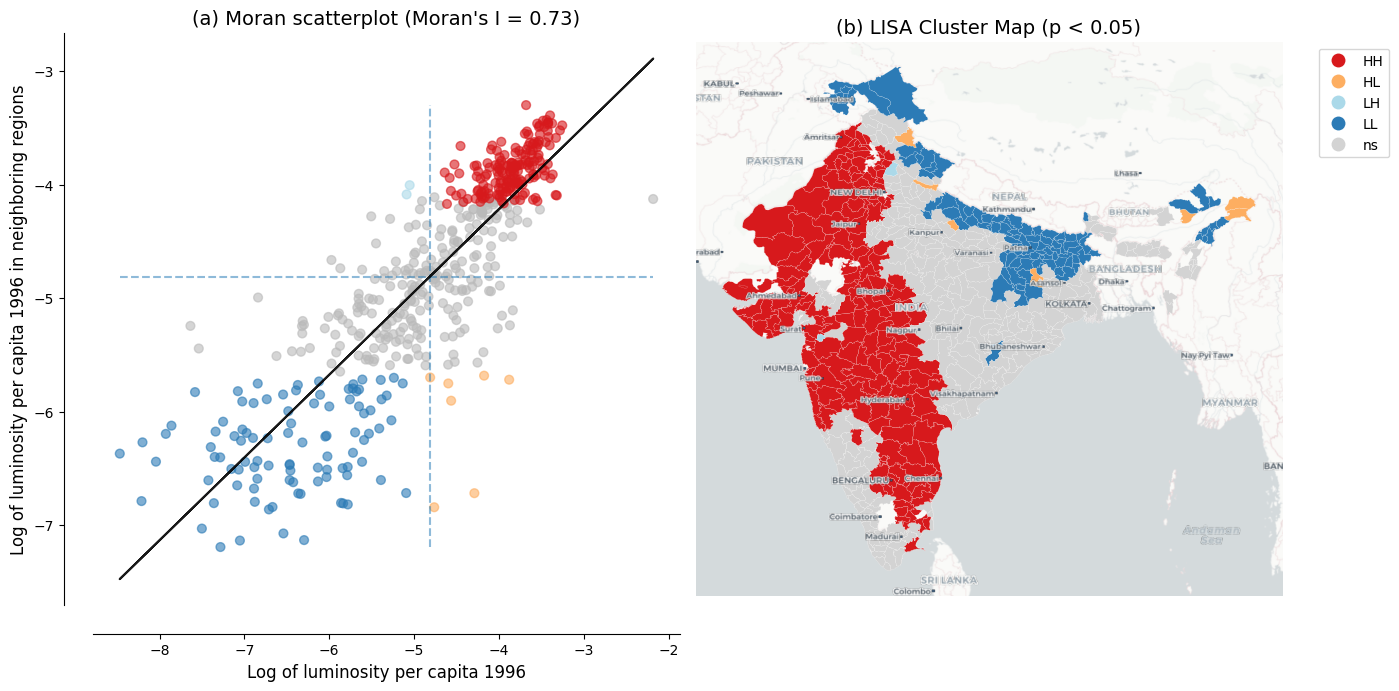
\includegraphics[keepaspectratio]{index_files/figure-latex/notebooks-c03_spatial_dependence_lisa-fig-dependence-initial-output-1.png}}

}

\caption{\label{fig-dependence-initial}Spatial dependence in the initial
level of luminosity Notes: Panel (a) shows the Moran scatterplot with
Global Moran's I statistic. Panel (b) shows the LISA cluster map with
statistically significant clusters at p \textless{} 0.05 based on 999
permutations. Source: Data from Chanda and Kabiraj (2020). See
\href{notebooks/c03_spatial_dependence_lisa.ipynb}{Spatial dependence}
notebook for source code.}

\end{figure}%

\textsubscript{Source:
\href{https://quarcs-lab.github.io/project2025s/notebooks/c03_spatial_dependence_lisa.ipynb.html\#cell-fig-dependence-initial}{Setup}}

The same LISA analysis applied to luminosity growth rates reveals a
geographic pattern that is largely the inverse of the initial luminosity
clusters, as shown in Figure~\ref{fig-dependence-growth}. Regions that
were classified as HH clusters in initial luminosity---the brightest
districts and their neighbors---tend to appear as LL clusters in
luminosity growth, indicating that these initially prosperous areas
experienced relatively slower growth over the study period. Conversely,
districts that formed LL clusters in initial luminosity---the dimmest
regions---tend to emerge as HH clusters in growth, reflecting faster
catch-up growth in initially lagging areas. This spatial inversion
between the initial level and subsequent growth of luminosity is the
spatial signature of the convergence process: initially red regions in
the luminosity map become blue regions in the growth map, and vice
versa. These local spatial patterns provide visual evidence that spatial
dependence is a prominent feature of the regional convergence process
observed in India, motivating the use of spatial econometric methods to
formally account for these inter-district spillovers in the analysis
that follows.

\begin{figure}[H]

\centering{

\pandocbounded{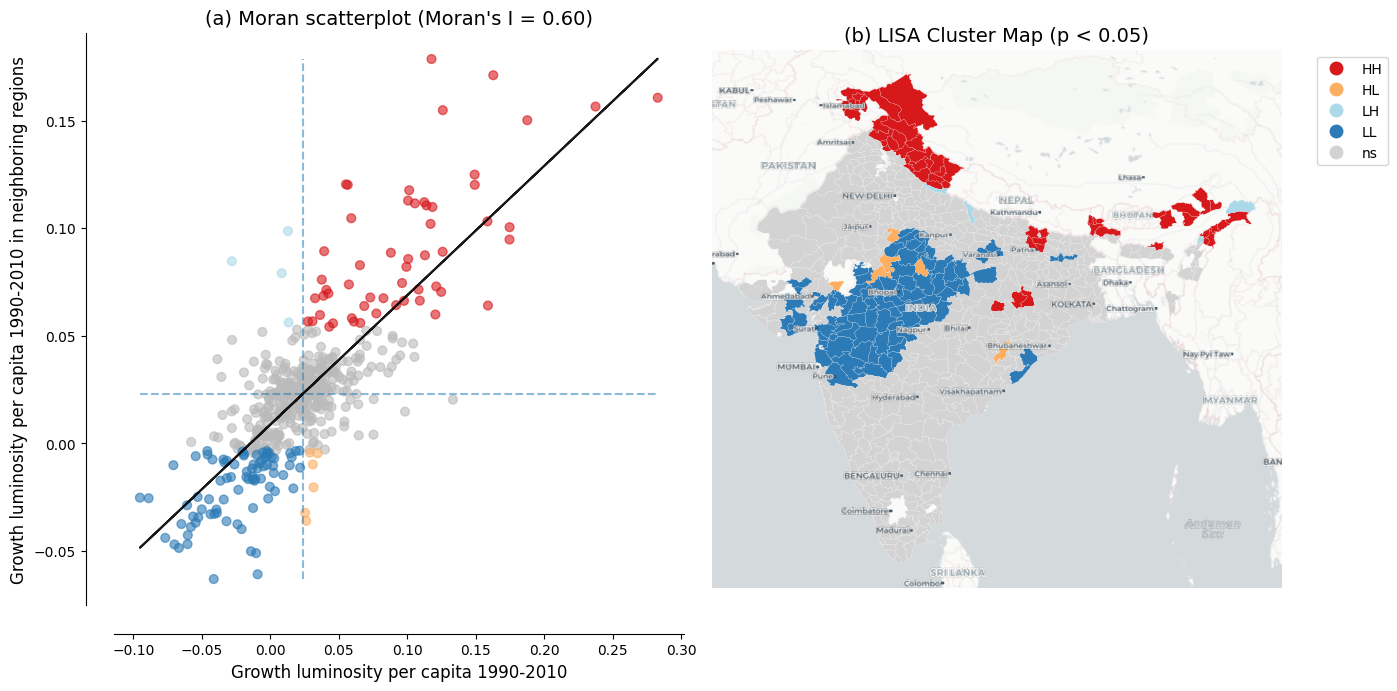
\includegraphics[keepaspectratio]{index_files/figure-latex/notebooks-c03_spatial_dependence_lisa-fig-dependence-growth-output-1.png}}

}

\caption{\label{fig-dependence-growth}Spatial dependence in the growth
rate of luminosity Notes: Panel (a) shows the Moran scatterplot with
Global Moran's I statistic. Panel (b) shows the LISA cluster map with
statistically significant clusters at p \textless{} 0.05 based on 999
permutations. Source: Data from Chanda and Kabiraj (2020). See
\href{notebooks/c03_spatial_dependence_lisa.ipynb}{Spatial dependence}
notebook for source code.}

\end{figure}%

\textsubscript{Source:
\href{https://quarcs-lab.github.io/project2025s/notebooks/c03_spatial_dependence_lisa.ipynb.html\#cell-fig-dependence-growth}{Setup}}

\subsection{Evidence of spatial spillovers in regional
convergence}\label{evidence-of-spatial-spillovers-in-regional-convergence}

The regression results of Table~\ref{tbl-models} provide evidence of
both unconditional and conditional convergence across districts in
India, with both conventional OLS and spatial econometric approaches
indicating significant negative relationships between initial luminosity
levels and subsequent growth rates. The direct effects, representing
within-district convergence, remain stable across specifications,
ranging from -0.020 to -0.026. This consistency across different model
specifications and estimation methods provides evidence that poorer
districts are catching up to their wealthier counterparts, even after
controlling for various district characteristics and state-level fixed
effects.

\begin{longtable}[]{@{}
  >{\raggedright\arraybackslash}p{(\linewidth - 16\tabcolsep) * \real{0.1282}}
  >{\raggedright\arraybackslash}p{(\linewidth - 16\tabcolsep) * \real{0.1154}}
  >{\raggedright\arraybackslash}p{(\linewidth - 16\tabcolsep) * \real{0.0897}}
  >{\raggedright\arraybackslash}p{(\linewidth - 16\tabcolsep) * \real{0.1154}}
  >{\raggedright\arraybackslash}p{(\linewidth - 16\tabcolsep) * \real{0.1154}}
  >{\raggedright\arraybackslash}p{(\linewidth - 16\tabcolsep) * \real{0.1154}}
  >{\raggedright\arraybackslash}p{(\linewidth - 16\tabcolsep) * \real{0.0897}}
  >{\raggedright\arraybackslash}p{(\linewidth - 16\tabcolsep) * \real{0.1154}}
  >{\raggedright\arraybackslash}p{(\linewidth - 16\tabcolsep) * \real{0.1154}}@{}}
\caption{Unconditional and conditional convergence across
districts.}\label{tbl-models}\tabularnewline
\toprule\noalign{}
\begin{minipage}[b]{\linewidth}\raggedright
\end{minipage} & \begin{minipage}[b]{\linewidth}\raggedright
Model 1
\end{minipage} & \begin{minipage}[b]{\linewidth}\raggedright
\end{minipage} & \begin{minipage}[b]{\linewidth}\raggedright
Model 2
\end{minipage} & \begin{minipage}[b]{\linewidth}\raggedright
\end{minipage} & \begin{minipage}[b]{\linewidth}\raggedright
Model 3
\end{minipage} & \begin{minipage}[b]{\linewidth}\raggedright
\end{minipage} & \begin{minipage}[b]{\linewidth}\raggedright
Model 4
\end{minipage} & \begin{minipage}[b]{\linewidth}\raggedright
\end{minipage} \\
\midrule\noalign{}
\endfirsthead
\toprule\noalign{}
\begin{minipage}[b]{\linewidth}\raggedright
\end{minipage} & \begin{minipage}[b]{\linewidth}\raggedright
Model 1
\end{minipage} & \begin{minipage}[b]{\linewidth}\raggedright
\end{minipage} & \begin{minipage}[b]{\linewidth}\raggedright
Model 2
\end{minipage} & \begin{minipage}[b]{\linewidth}\raggedright
\end{minipage} & \begin{minipage}[b]{\linewidth}\raggedright
Model 3
\end{minipage} & \begin{minipage}[b]{\linewidth}\raggedright
\end{minipage} & \begin{minipage}[b]{\linewidth}\raggedright
Model 4
\end{minipage} & \begin{minipage}[b]{\linewidth}\raggedright
\end{minipage} \\
\midrule\noalign{}
\endhead
\bottomrule\noalign{}
\endlastfoot
& OLS & SDM & OLS & SDM & OLS & SDM & OLS & SDM \\
Direct & -0.020*** & -0.021*** & -0.022*** & -0.021*** & -0.025*** &
-0.026*** & -0.025*** & -0.025*** \\
& (0.002) & (0.002) & (0.003) & (0.002) & (0.003) & (0.002) & (0.003) &
(0.002) \\
Indirect & -- & -0.001 & -- & -0.001 & -- & -0.015* & -- & -0.012* \\
& & (0.006) & & (0.005) & & (0.008) & & (0.007) \\
Total & -0.020*** & -0.022*** & -0.022*** & -0.022*** & -0.025*** &
-0.041*** & -0.025*** & -0.037*** \\
& (0.002) & (0.006) & (0.003) & (0.005) & (0.003) & (0.008) & (0.003) &
(0.007) \\
Controls & No & No & No & No & Yes & Yes & Yes & Yes \\
State FE & No & No & Yes & Yes & No & No & Yes & Yes \\
AIC & -1945 & -2290 & -2413 & -2466 & -2211 & -2356 & -2469 & -2499 \\
\end{longtable}

The progression from unconditional to conditional specifications reveals
how the estimated convergence process is shaped by the inclusion of
additional covariates. In the simplest unconditional models (Models 1
and 2), direct effects range from -0.020 to -0.022, while in the
conditional models that incorporate district-level controls (Models 3
and 4), direct effects increase in magnitude to -0.025 and -0.026. This
pattern suggests that omitting district characteristics attenuates the
estimated speed of convergence, and that once we account for structural
differences across districts---such as population density, urbanization,
or sectoral composition---the underlying tendency for poorer districts
to catch up becomes more pronounced. The inclusion of state fixed
effects, which capture unobserved state-level heterogeneity such as
differences in governance and institutional quality, further sharpens
the estimates by absorbing variation that might otherwise confound the
convergence relationship.

Importantly, the spatial Durbin model reveals spatial spillover effects
that are not captured by traditional OLS estimations. These indirect
effects, which capture the influence of neighboring districts' initial
conditions on a district's growth rate, follow a revealing pattern
across specifications. In the unconditional models (Models 1 and 2), the
estimated indirect effects are negligible and statistically
insignificant (-0.001 in both cases), suggesting that without proper
controls, spatial spillovers are confounded with omitted variables.
However, once district-level controls are introduced (Models 3 and 4),
the indirect effects become both larger in magnitude and statistically
significant, reaching -0.015 in Model 3 and -0.012 in our most
comprehensive Model 4. This emergence of significant spillover effects
in the conditional specifications indicates that identifiable spatial
channels of convergence---through which the economic conditions of
neighboring districts influence local growth---become identifiable only
after accounting for district-specific characteristics.

The total impact of initial conditions on growth, combining both direct
and spillover effects, is substantially larger when we account for
spatial dependence. In our fully specified model (Model 4), the total
convergence effect in the spatial Durbin model (-0.037) is approximately
48\% larger than the OLS estimate (-0.025). This gap is even more
pronounced in Model 3, where the SDM total effect (-0.041) exceeds the
corresponding OLS estimate (-0.025) by 64\%, highlighting that spatial
spillovers can constitute a substantial share of the overall convergence
process. These differences indicate that conventional non-spatial
approaches may significantly underestimate the speed of regional
convergence by failing to capture the additional convergence channels
created through spatial spillovers.

The model fit statistics further support the spatial econometric
approach. The Akaike Information Criterion (AIC) consistently favors the
spatial Durbin model over OLS across all four specifications, with the
most comprehensive model (Model 4 SDM) achieving the lowest AIC value of
-2499 compared to -2469 for the corresponding OLS. Notably, the
improvement from incorporating spatial structure is most pronounced in
the unconditional specification (Model 1), where the AIC drops by 345
units when moving from OLS to SDM, reflecting the large amount of
spatial dependence left unmodeled by ordinary regression. Even in the
fully specified model, where state fixed effects already absorb much of
the spatial heterogeneity, the SDM retains a meaningful advantage. Taken
together, these results suggest that regional convergence in India
operates not only through district-specific factors but also through
spatial interactions between neighboring districts, and that ignoring
these interactions leads to both underestimated convergence speeds and
inferior model performance.

\section{Discussion}\label{discussion}

\subsection{Better luminosity data from
VIIRS}\label{better-luminosity-data-from-viirs}

Our analysis, following \citet{chanda_kabiraj_district_convergence},
relies on radiance-calibrated DMSP-OLS nighttime lights data covering
the period 1996 to 2010. This dataset has been widely validated as a
proxy for economic activity
\citep{henderson_storeygard_weil_lights, chen_nordhaus_luminosity_gdp}.
Nevertheless, DMSP-OLS data suffer from well-documented limitations
including top-coding in bright urban cores, lack of on-board calibration
leading to inter-satellite inconsistencies, and blooming artifacts that
spatially blur light sources beyond their true boundaries
\citep{abrahams_etal_deblurring}. These measurement issues can attenuate
the precision of convergence estimates, particularly in rapidly
urbanizing districts where saturation may mask growth variation.

The Visible Infrared Imaging Radiometer Suite (VIIRS) Day/Night Band,
operational since 2012, represents a substantial improvement over
DMSP-OLS along multiple dimensions. VIIRS offers finer spatial
resolution (approximately 750 meters versus 2.7 kilometers), on-board
radiometric calibration that provides consistent quantitative
measurements, and a wider dynamic range that avoids saturation in urban
areas while detecting dim lights in rural settlements
\citep{elvidge_etal_viirs}. Comparative evaluations have shown that
VIIRS explains 10 to 15 percentage points more variation in subnational
economic activity than DMSP-OLS \citep{chen_nordhaus_measurement_error}.
Systematic assessments recommend VIIRS as the preferred product for
cross-sectional and recent time-series studies
\citep{gibson_etal_ntl_measurement}. Future extensions of our
convergence analysis using VIIRS data could yield more precise estimates
of both direct and indirect effects, particularly in districts where
DMSP saturation may have compressed the measured distribution of
luminosity.

A practical challenge for extending long-run convergence studies is the
discontinuity between DMSP (1992--2013) and VIIRS (2012--present) sensor
eras. Recent harmonization efforts, notably the global harmonized
nighttime light dataset by \citet{li_etal_harmonization}, have created
consistent 27-year time series by calibrating VIIRS observations to
DMSP-equivalent units during the overlap period. Such harmonized
datasets could enable the extension of our spatial Durbin analysis to
more recent periods, allowing researchers to examine whether the
convergence patterns and spatial spillovers documented here have
persisted, accelerated, or changed in character as India's economy has
continued to transform.

\subsection{New research directions}\label{new-research-directions}

While our analysis documents the average convergence effect and its
spatial spillover component, the cross-sectional regression framework
does not capture potential heterogeneity in convergence patterns across
the income distribution. Distribution dynamics approaches, as pioneered
by \citet{quah_twin_peaks}, could reveal whether Indian districts are
converging to a single steady state or forming distinct convergence
clubs where districts converge within groups but diverge across them.
The regression tree methods developed by
\citet{durlauf_johnson_convergence_clubs} for identifying multiple
growth regimes could be combined with spatial econometric techniques to
examine whether geographic clusters of districts follow distinct
convergence trajectories, potentially revealing spatial poverty traps or
growth poles that are not visible in average convergence estimates
\citep{rey_spatial_dynamics}. Indeed, satellite nighttime light data
have already been used to document convergence clubs and spatial
dependence across subnational regions in ASEAN
\citep{mendez_santos_asean_lights}, while convergence club methods have
revealed distinct growth regimes across Indonesian districts
\citep{aginta_etal_indonesia_clubs} and structural convergence patterns
across European regions \citep{cutrini_mendez_eu_clubs}. Furthermore,
analysis of harmonized luminosity data across Chinese provinces has
uncovered complex inequality dynamics that differ markedly across
cross-sectional and temporal dimensions
\citep{glawe_mendez_china_luminosity}. Extending these multi-country
insights to the Indian district context could help determine whether the
convergence patterns we document reflect a single equilibrium or mask
the formation of distinct spatial clubs.

A second important direction concerns the causal identification of the
spillover channels that our spatial Durbin model captures in reduced
form. While our estimates document significant indirect effects, the
model does not identify whether these spillovers operate through
infrastructure linkages, labor migration, technology diffusion, or
market access channels. Quasi-experimental approaches, such as those
employed by \citet{asher_novosad_rural_roads} to study the causal
effects of rural road construction on structural transformation in
India, could be embedded within spatial econometric frameworks to
isolate specific spillover mechanisms. Understanding which channels
drive the indirect convergence effects is important for designing
spatially targeted policies that may amplify positive spillovers.
Comparative evidence from other developing economies suggests that
spatial dependence in regional convergence is a widespread phenomenon
rather than an India-specific feature. Studies have documented
significant spatial spillover effects in convergence processes across
Thailand \citep{tipayalai_mendez_thailand}, Turkey
\citep{ursavas_mendez_turkey}, and Indonesian districts
\citep{miranti_mendez_indonesia}, with neighbor effects and spatial
conditioning factors playing important roles in shaping convergence
trajectories. This cross-country regularity strengthens the case for
systematic investigation of the specific mechanisms driving spatial
spillovers, as the channels may differ across institutional and
geographic contexts.

Third, the growing availability of diverse satellite products and
machine learning methods opens possibilities for richer measurement of
regional economic activity. \citet{jean_etal_poverty_prediction}
demonstrated that combining high-resolution daytime imagery with
nighttime lights through deep learning can substantially improve poverty
prediction in data-scarce settings. Similarly,
\citet{keola_etal_lights_poverty} showed that integrating nighttime
lights with land cover data improves economic measurement in
agricultural areas where lights alone provide weak signals. As
\citet{donaldson_storeygard_remotesensing} emphasize, the expanding
ecosystem of satellite-derived data---including vegetation indices,
built-up area detection, and high-frequency mobility indicators---offers
opportunities to construct multi-dimensional proxies for regional
economic activity that go beyond what nighttime lights alone can
capture. Recent applications demonstrate the practical potential of
these advances for subnational economic measurement.
\citet{chen_etal_turkey_viirs} show that higher-quality VIIRS nighttime
lights can predict sectoral GDP composition across Turkish provinces,
distinguishing between urban service-oriented and rural agricultural
regions in ways that DMSP data cannot. \citet{hussein_etal_vietnam_ml}
employ machine learning methods with multiple remote sensing indicators
to predict subnational GDP in Vietnam, achieving accuracy improvements
over traditional luminosity-based approaches. At a broader scale,
\citet{theara_etal_cambodia_poverty} combine big data sources,
socioeconomic surveys, and machine learning to map multidimensional
poverty in Cambodia, illustrating how satellite-derived features can
complement conventional survey instruments. Applying similar
multi-source approaches to Indian districts could yield richer proxies
for economic activity that overcome the well-known limitations of
nighttime lights in agricultural and low-density areas.

\subsection{Research reproducibility and open
science}\label{research-reproducibility-and-open-science}

The complexity of satellite-based economic research---involving
multi-step data processing pipelines, spatial econometric estimation,
and geographic visualization---makes reproducibility both challenging
and essential. As \citet{donaldson_storeygard_remotesensing} note, the
processing of satellite data requires careful documentation and sharing
of code to ensure that results can be replicated and extended. Each
methodological choice in the pipeline, from sensor inter-calibration to
spatial weight matrix construction, can affect empirical conclusions,
underscoring the need for transparent computational workflows that allow
other researchers to verify and build upon published findings
\citep{gibson_etal_ntl_measurement}.

This article adopts a reproducible research approach through Quarto's
single-source publishing framework, where a single manuscript file
generates multiple output formats---interactive HTML, journal PDF, and
supplementary materials---from the same source. All computational
analyses are documented in embedded notebooks that readers can inspect
alongside the results they produce, creating a complete chain from raw
data to published findings. The interactive web-based visualization
tool, built on Google Earth Engine, allows researchers to independently
explore the spatial and temporal patterns in the nighttime light data,
facilitating verification of our visual findings and supporting further
exploration beyond what static representations can convey.

Open-source tools and cloud computing platforms are rapidly lowering the
barriers to reproducible spatial economic research. Cloud-based
computational notebooks, such as those developed by
\citet{mendez_patnaik_notebook} for processing nighttime lights data,
eliminate the need for specialized local software and provide accessible
workflows for data ingestion, preprocessing, spatial analysis, and
visualization. The combination of open data repositories,
version-controlled code, and cloud computing infrastructure creates an
ecosystem where the full analytical pipeline---from satellite imagery to
econometric results---can be made transparent, verifiable, and
extensible by the broader research community.

\section{Concluding remarks}\label{concluding-remarks}

This article examines regional convergence patterns across Indian
districts using satellite nighttime light data, interactive
visualizations, and spatial econometric modeling. Building on the work
of \citet{chanda_kabiraj_district_convergence}, we developed an
interactive web-based visualization tool that illustrates spatial and
convergence patterns across Indian districts. Spatial autocorrelation
tests indicate that spatial dependence is a notable characteristic of
satellite data and the regional convergence process in India. Estimates
from our spatial Durbin model indicate that incorporating spatial
spillovers increases the estimated speed of regional convergence. The
total convergence effect in our fully specified model is approximately
48\% larger than conventional non-spatial estimates. This finding
suggests that non-spatial convergence models may underestimate the speed
of regional convergence. Additionally, it suggests that place-based
development interventions may have broader impacts, as their benefits
can extend to neighboring districts through spatial spillover effects.

Our analysis underscores the value of satellite nighttime lights as a
tool for studying economic dynamics in countries where subnational data
are scarce, infrequent, or unreliable. Conventional economic statistics
at the district level are often unavailable or inconsistent across
administrative boundaries, particularly in large developing economies.
Radiance-calibrated nighttime light data allowed us to analyze 520
Indian districts at a spatial granularity that would be difficult to
achieve with traditional national accounts or survey data alone. This
data-driven approach is potentially transferable to other data-poor
contexts across the developing world, and the ongoing transition from
DMSP-OLS to the higher-resolution VIIRS sensor promises even more
precise measurement of subnational economic activity in future studies.

The spatial modeling framework employed in this study illustrates the
complementary insights that emerge from layering different analytical
approaches. Interactive visualizations built on Google Earth Engine
enabled an initial exploratory examination of spatial and temporal
patterns in luminosity, making the geographic dimension of convergence
accessible to a broad audience. Exploratory spatial data analysis
through Global Moran's I and LISA statistics then formalized these
visual impressions, confirming strong positive spatial autocorrelation
in both initial luminosity levels (\(I = 0.73\)) and subsequent growth
rates (\(I = 0.60\)), and identifying the specific geographic clusters
driving these patterns. Finally, the spatial Durbin model provided a
formal econometric framework to quantify spillover effects and indicate
that convergence speeds may be underestimated when spatial interactions
are ignored. Together, these three layers form a coherent analytical
pipeline---from visual exploration to formal statistical testing to
spatial econometric modeling---that captures dimensions of the
convergence process not addressed by conventional non-spatial methods.

This study also illustrates how reproducible open science practices can
strengthen the credibility and impact of spatial economic research. The
entire analytical pipeline---from raw satellite data to published
findings---is documented in computational notebooks using Python, R, and
Stata, all embedded within the manuscript through Quarto's single-source
publishing framework. A single manuscript source generates multiple
output formats, including an interactive HTML version that allows
readers to inspect the underlying code and results alongside the text.
The interactive Google Earth Engine application provides an additional
layer of verification, enabling independent exploration of the spatial
and temporal patterns discussed in the article. By hosting the complete
codebase in a public repository and making the notebooks executable
through cloud-based platforms, we aim to lower the barriers to
replication and extension, offering this workflow as a potential
template for other researchers working at the intersection of remote
sensing and spatial economics.

From a policy standpoint, these results suggest that regional
convergence operates not just through district-specific factors, but
through complex spatial interactions that create additional channels for
catch-up growth. The significant spatial spillover effects uncovered by
the spatial Durbin model imply that place-based development
interventions may generate benefits beyond their immediate target areas,
as improvements in one district can positively influence the growth
trajectories of neighboring districts. Understanding the magnitude of
these spatial multiplier effects is important for the design and
evaluation of regional development programs aimed at reducing spatial
inequalities. More broadly, the combination of new data sources, spatial
analytical methods, and open science practices illustrated in this
article offers a potentially useful framework for studying regional
economic disparities in developing countries.

\section{Acknowledgments}\label{acknowledgments}

This work was supported by JSPS KAKENHI Grant Number 24K04884. During
the preparation of this work, the authors used Claude Code (Anthropic)
to assist with manuscript editing, computational notebook development,
and research infrastructure setup. After using this tool, the authors
reviewed and edited all content and take full responsibility for the
content of the publication.

\section{Conflict of Interest}\label{conflict-of-interest}

The authors declare no conflict of interest.

\section{Data and Code Availability}\label{data-and-code-availability}

All data and computational code used in this study are available in the
project repository: \url{https://github.com/quarcs-lab/project2025s}.
Also, the interactive HTML version of this manuscript
(\url{https://quarcs-lab.github.io/project2025s/}) embeds the
computational notebooks, allowing readers to inspect the complete
analytical pipeline from raw data to published results.


\bibliography{references.bib}



% This is the COPYRIGHT statement for the article.
\vspace*{\fill}
\tabcolsep0mm
\noindent
\begin{tabular*}{\textwidth}{ll}
	\toprule
	\multirow{2}{19mm}{
\includegraphics[width=18mm,height=10mm]{_extensions/region-ersa/REGION/CC-BY-88x31}} & {\small \multirow{2}{328pt}{\textcopyright\  by the authors. Licensee: REGION -- The Journal of ERSA, European Regional Science Association, Louvain-la-Neuve, Belgium. This article is distri-}} \\
	& \\[-1pt]
	\multicolumn{2}{l}{\small \multirow{2}{\textwidth}{buted under the terms and conditions of the Creative Commons Attri\-bution (CC BY) license (\href{http://creativecommons.org/licenses/by/4.0/}{http://creativecommons.org/licenses/by/4.0/}).}}\\
	& \\
	\bottomrule
\end{tabular*}

\end{document}
